% Preamble
\documentclass[11pt,pdf, aspectratio=169]{beamer}
\usetheme{metropolis}

% Packages
\usepackage{amsmath}
\usepackage[utf8]{inputenc}
\usepackage[T1]{fontenc}
\usepackage{graphicx}
\usepackage{tikz}
\usepackage{minted}
\usepackage[
  type={CC},
  modifier={by-sa},
  version={4.0},
]{doclicense}
\usepackage{hyperref}
%\setsansfont{Fira Sans}
\usemintedstyle{manni}
\setminted{
  fontsize=\footnotesize,linenos,frame=lines, framesep=2mm
}

\title{FPC Training session}
\author{Verwoerd}
\date{April 30, 2023}
% Document
\begin{document}

  \section{Introduction}
  \begin{frame}{Welcome}
    \begin{itemize}
      \item Welcome to the FPC 2024 Introduction sessions
      \item 2 parts
      \item First Part gives introduction of programming contests
      \item We will discuss all last year's problems of the FPC in the second part
      \item Problem-set is available on paper, try to read through it in the break
    \end{itemize}
  \end{frame}
  \begin{frame}{Who am I}
    \begin{itemize}
      \item Alumnus, working in the Software Industry
      \item Involved in organizing programming contests since 2003 as volunteer
      \item ``Coach'' for TU Delft teams since NWERC 2003
      \item Twice coach on the World Finals
    \end{itemize}
    \doclicenseThis
  \end{frame}


  \section{Introduction to Programming Contests}
  \begin{frame}{What is a programming contest?}
    \begin{itemize}
      \item<1-> Team of 3 people
      \item<1-> Single computer
      \item<1-> Solve as many problems from the problem set (8 to 15 problems)
      \item<1-> In 5 hours
      \item<1-> In any order
      \begin{itemize}
        \item<2-> Solve it efficiently
        \item<2-> do it as quickly as possible (under pressure)
        \item<2-> and do it correctly (without bugs)
      \end{itemize}
      \item<3-> With limited documentation and no internet
    \end{itemize}
  \end{frame}
  \begin{frame}{How is score calculated?}
    \begin{itemize}
      \item<1-> Sorted by number of problems solved
      \item<2-> Sorted by the total time for solved problems
      \begin{itemize}
        \item<3->  Time in minutes since the start of the contest
        \item<3-> Penalty for each wrong attempt on a solved solution of 20 minutes
        \begin{itemize}
          \item<4-> Penalty time is counts only if the problem is solved afterward.
          \item<4-> Penalty time does not reduce your contest time.
          \item<4-> Penalty time is not added after wrong attempts after the problem is solved.
          \item<4-> No penalty for compiler errors.
        \end{itemize}
      \end{itemize}
    \end{itemize}
  \end{frame}
  {
    \setbeamertemplate{background canvas}{
      \includegraphics[height=\paperheight]{images/session-1/scoreboard}
    }
    \begin{frame}{Example Scoreboard}
    \end{frame}
  }

  \begin{frame}{Freshman Programming Contest (FPC)}
    \begin{itemize}
      \item Contest of 3 hours
      \item Simpler problems
      \item preparation for the Delft Algorithm Programming Contest (DAPC)
    \end{itemize}
  \end{frame}
  \begin{frame}{Delft Algorithm Programming Contest (DAPC)}
    \begin{itemize}
      \item Contest is 5 hours instead of 3
      \item Official preliminary for International Collegiate Programming Contest (ICPC)
      \item Increased difficulty in every contest
    \end{itemize}
  \end{frame}
  \begin{frame}{Road to the world finals}
    The DAPC is an official preliminary of the ICPC.
    \begin{tikzpicture}
  \tikzstyle{every node}=[draw]
  \node {International Collegiate Programming Contest World Finals}
  child {node {NAC}}
  child {node{$\ldots$}}
    child {node[red]{EUC}} {
      child {node[red]{NWERC}
          child { node[red] {BAPC}
            child {node[red] {DAPC} edge from parent node[left, draw=none]{\textasciitilde 5 best teams}}
            child {node {AAPP}}
            child {node {EAPC}}
            child {node {TAPC}}
            child {node {$\ldots$}}
            edge from parent node[left, draw=none]{best teams per university}
          }
      child {node{GCPC}}
      child {node{NCPC}}
      child {node{UKIEPC}}
      edge from parent node[left, draw=none] {13 best teams}
    }
    child {node{CERC}}
    child {node{SWERC}}
    child {node{SEERC}}
  };

\end{tikzpicture}

  \end{frame}


  \section{Reading a problem}
  \begin{frame}{Problem structure}
    A typical problem has the following structure
    \begin{itemize}
      \item Problem description
      \item Input description
      \item Output description
      \item Example input/output
      \item A time limit in seconds
    \end{itemize}
    You are asked to write a program that solves the problem for all valid inputs within the time limit.
  \end{frame}
  \begin{frame}{Example problem}
    \begin{block}{Problem description}
      Write a program that multiplies pairs of integers.
    \end{block}
    \vspace{10pt}
    \begin{block}{Input description}
      The input consists of:
      \begin{itemize}
        \item One line with an integer $t$ ($1\leq t\leq 100$), the number of test cases.
        \item $t$ lines, each with two integers $a$ and $b$ ($|a|,|b| \leq 10^6$), the numbers to multiply.
      \end{itemize}
    \end{block}

    \vspace{10pt}

    \begin{block}{Output description}
      For each test case, output the value of $a\times b$.
    \end{block}
  \end{frame}
  \begin{frame}{Example problem}
    \begin{center}
      \begin{tabular}{|l|l|}
        \hline
        {\footnotesize Sample input} & {\footnotesize Sample output} \\
        \hline
        \begin{minipage}{80pt}
          \vspace{10pt}
          \ttfamily
          4\\
          3 4\\
          13 0\\
          1 8\\
          100 100\\
        \end{minipage}
        &
        \begin{minipage}{80pt}
          \vspace{10pt}
          \ttfamily
          12\\
          0\\
          8\\
          10000\\
        \end{minipage}
        \\
        \hline
      \end{tabular}
    \end{center}
  \end{frame}
  \begin{frame}[containsverbatim]{Solution in C++}
    \inputminted{c++}{code/session-1/c++/example-wrong.cpp}
  \end{frame}
  \begin{frame}[containsverbatim]{Solution in Java}
    \inputminted{java}{code/session-1/java/example-wrong.java}
  \end{frame}
  \begin{frame}[containsverbatim]{Solution in Kotlin and Python}
    \inputminted{kotlin}{code/session-1/kotlin/example-wrong.kt}
    \inputminted{python}{code/session-1/python/example.py}
  \end{frame}


  \section{Introduction to DOMJudge}
  \begin{frame}{Submitting the Solution}
    \begin{itemize}
      \item During the contest you submit to a contest control system
      \begin{itemize}
        \item Usually DOMJudge, but sometimes Kattis or PC\textasciicircum2
      \end{itemize}
      \item Submit solutions
      \item Ask questions about the problems or programming environment
      \item Read clarifications from the jury
    \end{itemize}
  \end{frame}
  \begin{frame}{Domjudge Interface - home}
    \includegraphics[width=\linewidth]{images/session-1/domjudge-initial}
  \end{frame}
  \begin{frame}{Domjudge Interface - problems}
    \includegraphics[width=\linewidth]{images/session-1/domjudge-problems}
  \end{frame}
  \begin{frame}{Domjudge Interface - submit}
    \includegraphics[width=\linewidth]{images/session-1/domjudge-submit}
  \end{frame}
  \begin{frame}{Are the solutions correct?}
    \includegraphics[width=\linewidth]{images/session-1/domjudge-submit-first-try}
  \end{frame}
  \begin{frame}{We made a whoopsy?}
    \includegraphics[width=\linewidth]{images/session-1/domjudge-no-double}
  \end{frame}
  \begin{frame}{Or not}
    \includegraphics[width=\linewidth]{images/session-1/domjudge-correct}
  \end{frame}
  \begin{frame}{Lets ask the jury}
    \includegraphics[width=\linewidth]{images/session-1/domjudge-clar-1}
  \end{frame}
  \begin{frame}{Lets hope they respond fast}
    \includegraphics[width=\linewidth]{images/session-1/domjudge-clar-2}
  \end{frame}
  \begin{frame}{We have a response}
    \includegraphics[width=\linewidth]{images/session-1/domjudge-clar-3}
  \end{frame}
  \begin{frame}{The jury is not helping us}
    \includegraphics[width=\linewidth]{images/session-1/domjudge-clar-4}
  \end{frame}
  \begin{frame}{Why did the 3 solutions fail?}
    \begin{itemize}
      \item <1-> Lets check the input again: $|a|,|b| \leq 10^6$
      \item <2-> Worst case scenario: $a=10^6$ and $b=10^6$ giving  $a \times b = 10^{12}$
      \item <3-> Does $10^{12}$ fit in a 32-bit \texttt{int}?
      \item <4-> $\log_2 10^{12} \approx 40$, so \textbf{NO}, 40 bits don't fit in an \texttt{int}
      \item <5-> Use \texttt{long (long)} when possible, except in Python
    \end{itemize}
  \end{frame}
  \begin{frame}[containsverbatim]{Solution in C++}
    \inputminted{c++}{code/session-1/c++/example.cpp}
  \end{frame}
  \begin{frame}[containsverbatim]{Solution in Java}
    \inputminted{java}{code/session-1/java/example.java}
  \end{frame}
  \begin{frame}[containsverbatim]{Solution in Kotlin}
    \inputminted{kotlin}{code/session-1/kotlin/example.kt}
  \end{frame}
  \begin{frame}{All solutions correct}
    \includegraphics[width=\linewidth]{images/session-1/domjudge-all-correct}
  \end{frame}


  \section{Estimating problem complexity}
  \begin{frame}{About time limit}
    \begin{itemize}
      \item The time limit specifies the time you program may run
      \item This includes JVM-startup and I/O
      \item High time limit signify \begin{itemize}
                                      \item lots of I/O
                                      \item Slower algorithms can be accepted
      \end{itemize}
      \item Low limit signifies fast algorithms, usually the use of formulas
      \item You can use the time limit to check your code on your local machine\\
      \texttt{\$ time myjava ProblemA < worst-case.in}
    \end{itemize}
  \end{frame}
  \begin{frame}{About input size\footnote[1]{https://gcpc.nwerc.eu/primer.pdf}}
    Based on the input size you can an idea of the time complexity.

    \begin{center}
      \begin{tabular}{llll}
        \hline
        $\mathcal{O}(n!)$         & $n \leq 10$   & $\mathcal{O}(n\log{}^{2}n)$ & $n \leq 10^5$    \\
        $\mathcal{O}(2^n)$        & $n \leq 20$   & $\mathcal{O}(n\log{}n)$     & $n \leq 10^6$    \\
        $\mathcal{O}(n^3)$        & $n \leq 500$  & $\mathcal{O}(n)$            & $n \leq 10^8$    \\
        $\mathcal{O}(n^2\log{}n)$ & $n \leq 1000$ & $\mathcal{O}(\sqrt{n})$     & $n \leq 10^{15}$ \\
        $\mathcal{O}(n^2)$        & $n \leq 5000$ & $\mathcal{O}(\log{}n)$      & $n \leq 10^{18}$ \\
        $\mathcal{O}(n\sqrt {n})$ & $n \leq 10^5$ &                             &                  \\
        \hline
      \end{tabular}
    \end{center}

    \textbf{Warning}: This is not guaranteed to be always the case!
  \end{frame}


  \section{Tips, tricks and common mistakes}
  \begin{frame}{General tips}
    \begin{itemize}
      \item Read the output specification carefully!
      \item Don’t forget to remove debug prints!
      \item When integers get large, use 64-bit!
      \item Do not do string concatenation with $+$ in a loop!
      \item Calling functions is more expensive than you might think!
      \item For Java, \texttt{BufferedReader} is faster than \texttt{Scanner}!
      \item Don’t forget to eat and drink.
      Programming contest is a sport, and you need to be energized and focussed for the whole contest.
    \end{itemize}
  \end{frame}

  \begin{frame}{Selecting the first problem}
    \begin{itemize}
      \item Decide on a reading tactic
      \begin{itemize}
        \item Do we all start reading the first problem?
        \item Or does one person start at the end?
      \end{itemize}
      \item There are usually several ``simple'' problems in a set
      \item Be careful: the easiest problems usually contain some pitfall corner cases!
    \end{itemize}
  \end{frame}
  \begin{frame}{Finding the easiest problems by results}
    \begin{itemize}
      \item After a few minutes of contest, the first balloons will be handed out
      \item Check the scoreboard or balloon colours to see which problem is solved most\\
      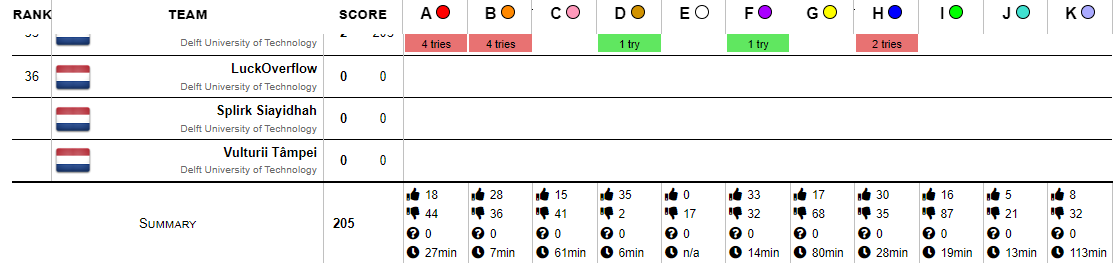
\includegraphics[width=\linewidth]{images/session-2/bottom-scoreboard}
      \item Or the problems page in DOMJudge (only newer versions)
      \item \textbf{Warning}: The first problem solved is not guaranteed the easiest!
    \end{itemize}
  \end{frame}
  \begin{frame}{My problem is wrong, what now}
    Print out the problem and let other people work on the computer, work out cases that might go wrong.
    \begin{itemize}
      \item When the result is RTE:
      \begin{itemize}
        \item Check for possible null pointers, array overflows, or integer overflow
        \item Check the input specification, don't forget 0 can do unexpected things
      \end{itemize}
      \item When the result is TLE:
      \begin{itemize}
        \item Check stop conditions, maybe an infinite loop?
        \item Code is too slow, try optimizing or thinking of a faster solution
      \end{itemize}
      \item When then result is WA:
      \begin{itemize}
        \item Check for corner cases, don't forget zero
        \item Check correctness of algorithm
      \end{itemize}
      \item \textbf{Warning}: A problem can be WA and TLE at the same time, but only \emph{one} is reported back!
    \end{itemize}
  \end{frame}
  \begin{frame}{Common Battle Plan}
    \begin{description}
      \item [Start of contest] Prepare computer, find and solve easiest problems, all problems should be read by at least a single team member.
      \item[First hours] Prioritize solving the easiest problems, every team member works on their own problems
      \item[Mid contest] Work on solving harder problems with 2 people, while the last person works alone on the last easy or specialized hard problems
      \item[End of the contest] Work together with the whole team on a single problem, free submit mode
    \end{description}
  \end{frame}
  \begin{frame}{Common Errors}
    \begin{itemize}
      \item Focus on the first problem you think you can solve
      \item Not reading all problems in the set
      \item Debugging on the computer while another solution can be implemented
      \item Fighting who can solve which problem
      \item Not rewriting code when it gets to messy
    \end{itemize}
  \end{frame}

  \begin{frame}{Training your self}
    \begin{itemize}
      \item If you want to try to make it to the World Finals, you can train for next year's DAPC
      \item Many online problem-solving websites:
      \begin{itemize}
        \item December: Advent of code (\url{https://adventofcode.com/})
        \item September-Januari: Universal Cup (\url{https://ucup.ac})
        \item Year round: Kattis Problem Archive (\url{https://open.kattis.com/})
        \item Year round: Codeforces (\url{https://codeforces.com/})
      \end{itemize}
      \item Several books available, listed on \url{https://chipcie.wisv.ch/resources}
    \end{itemize}
  \end{frame}


  \section{FPC 2023 problems}\label{sec:fpc-2023-problems}
  \begin{frame}{Admiring Droplets}
    \begin{itemize}
      \item FPC 2023
      \item Time limit: 3s
      \item Difficulty: Very Easy
      \item Given $n$ droplets on the same vertical line with size $s (\mu L)$ on a window with distance $y$ ($mm$) from the top.
      The velocity is is given by $v = \sqrt[6]{V}$ ($v$ in $m/s$ and $V$ in $m^3$) and when two droplets meet they coalesce together ($V=s_{current}+s_{next}$).
      Calculate the time takes for the coalesced droplet to reach the bottom of the window using the
    \end{itemize}
    Original problem written by the FPC 2023 jury and licensed under \doclicenseLongNameRef.

    \doclicenseImage

  \end{frame}
  \begin{frame}{Admiring Droplets}
    \begin{itemize}
      \item<1-> \textbf{Observation:} $n \leq 10^5$, so we are looking for a $\mathcal{O}(n)$ solution
      \item<2-> Simulate the droplets from highest to lowest
      \item<3-> For the current droplet, calculate the time to reach the closest droplet
      \item<4-> Merge the droplets together and calculate the new size
      \item<4-> Repeat until a single droplet is left and print the sum of the time
      \item<4-> \textbf{Pitfall:} \begin{itemize}
                                    \item Be careful with unit conversion: $1m = 1000mm$, $1 m^3=10^{9}mm^3$
                                    \item Off by one errors
      \end{itemize}
    \end{itemize}
  \end{frame}
  \begin{frame}{Beaking Spackwards}
    \begin{itemize}
      \item FPC 2023
      \item Time limit: 1s
      \item Difficulty: Easy
      \item Given a input $s$, print a string containing exactly $s$ palindromes
    \end{itemize}
    Original problem written by the FPC 2023 jury and licensed under \doclicenseLongNameRef.

    \doclicenseImage

  \end{frame}
  \begin{frame}{Beaking Spackwards}
    \begin{itemize}
      \item<1-> \textbf{Observation:} $n \leq 10^9$, so we are looking for a solution faster $\mathcal{O}(n)$
      \item<2-> \textbf{Observation:} a string \texttt{"aaa...aaa"} of size $l$ has $\frac{l(l+1)}{2}$ palindromes
      \item<3->  The length of the word should be $\lceil\sqrt{n}\rceil$
      \item<4-> Find the largest $l$ where $l \leq n$ by search or using the formula $l = \lfloor\frac{\sqrt {8n + 1}-1}{2}\rfloor$\\\[
                                                                                                                                       \frac{l(l+1)}{2}\leq n \equiv l^2+l \leq 2n \equiv l^2+l-2n \leq 0 \equiv l \leq \frac{-1 + \sqrt {1+4\cdot 2n}}{2}\]
      \item<5-> Generate a string of length $l$ with the same letter that is unused
      \item<5-> or append a non palindrome letter to increase the number of palindromes is the desired size
      \item<5-> Update $n$ with the remaining length and repeat until $n=0$ and print the string
      \item<6-> \textbf{Pitfall:} Be careful with slow string concatenations
    \end{itemize}
  \end{frame}
  \begin{frame}{Catchy Tunes}
    \begin{itemize}
      \item FPC 2023
      \item Time limit: 3s
      \item Difficulty: Medium
      \item Given a list on $n$ songs with their artist, generate an ordering where every song is followed with a song from a different artist.
    \end{itemize}
    Original problem written by the FPC 2023 jury and licensed under \doclicenseLongNameRef.

    \doclicenseImage

  \end{frame}
  \begin{frame}{Beaking Spackwards}
    \begin{itemize}
      \item<1-> \textbf{Observation:} $n \leq 10^5$, so we are looking for a $\mathcal{O}(n)$ solutions
      \item<1-> At least half of the songs in her playlist are from a unique artist
      \item<2-> Group the songs in two lists during input if the artist is unique or not
      \item<3-> Alternate printing a song title from either list and remove it
      \item<3-> If one list is empty, keep printing from the other list
    \end{itemize}
  \end{frame}
  \begin{frame}{Dungeon of Darkness}
    \begin{itemize}
      \item FPC 2023
      \item Time limit: 1s
      \item Difficulty: Hard
      \item \textbf{Interactive Problem}
      \item Using interactions, navigate a maze and find the exit.
    \end{itemize}
    Original problem written by the FPC 2023 jury and licensed under \doclicenseLongNameRef.

    \doclicenseImage

  \end{frame}
  \begin{frame}{What are Interactive Problems?}
    \begin{itemize}
      \item Traditional problems give all the input at once, you solve and print all the output at once
      \item Interactive problems give input, you do work, print output, and you receive new input
      \item This process continues until you find the final answer
      \item The problem defines an interaction protocol
      \item The problem may have an interaction limit
      \item If an interactive problem may be in the set, an simple interactive problem will be included in the test session
    \end{itemize}
  \end{frame}
  \begin{frame}{Type of problems for Interactive Problems}
    \begin{itemize}
      \item Search in a finite space
      \item Explore a maze
      \item Matching games
      \item Double interaction problem (very, very rare)
      \begin{itemize}
        \item Program has 2 modes
        \item the first mode, input transforms input to output following certain rules
        \item The second mode, the output of mode 1 is given and you have tranform it back to the input of mode 1
      \end{itemize}
    \end{itemize}
  \end{frame}
  \begin{frame}{Common pitfalls for Interactive problems}
    \begin{itemize}
      \item Flush the output after every write
      \begin{itemize}
        \item Only the output, not the input
        \item Not flushing the output results in Time Limit Exceeded
      \end{itemize}
      \item Verdict of a solution is not deterministic, but the following is guaranteed:
      \begin{itemize}
        \item Wrong Answer means you printed something wrong
        \item Runtime Error means you returned an 0 error code
        \item If both occur, you will get either
      \end{itemize}
      \item ICPC style contests don't have ``Idleness Limit Exceeded'', but a total runtime limit.
    \end{itemize}
  \end{frame}
  \begin{frame}{Flushing the output}
    \begin{description}
      \item [C++]: end your output with \mintinline{c++}|std::endl| or \mintinline{c++}|std::flush|
      \item[Python]: use the flush parameter, like \mintinline{python}|print("abc", flush=True)|
      \item[Java/Kotlin]: use a \mintinline{java}|java.io.BufferedWriter| and after each write use the \mintinline{java}|.flush()| method.
    \end{description}
  \end{frame}
  \begin{frame}{Interactive problems testing tool}
    \begin{itemize}
      \item Most contests provide a testing tool to test the interaction with a testing tool
      \item This is usually called \texttt{testing\_tool.py} in our region
      \item The header file tells you how to run run the testing tool, for example\\\texttt{\textdollar{} python3 testing\_tool.py -f 1.in python3 ./solution.py}
      \item Pitfall for Java/Kotlin: You should run the testing tool in the directory which contains the compiled class file

      \item \textbf{Wrong}:\\\texttt{\textasciitilde/\textdollar{} python3 testing\_tool.py -f 1.in java ./code/ProblemA}
      \item \textbf{Right}:\\\texttt{\textasciitilde/code/\textdollar{} python3 testing\_tool.py -f 1.in java ProblemA}
    \end{itemize}
  \end{frame}
  \begin{frame}{Dungeon of Darkness}
    \begin{itemize}
      \item<1-> Get to the final room in a dungeon, where you only see the symbols of the doors leading from the current room.
      \item<2-> Use a Depth First Search (DFS) to delve deeper in the maze
      \item<3-> If the exit is in the room, go through to the exit
      \item<3-> If in a room, the exit is not there, move through a door you haven't visited yet
      \item<3-> If all doors are visited, move back to the door you entered the room through
    \end{itemize}
  \end{frame}
  \begin{frame}{Expected eyes}
    \begin{itemize}
      \item FPC 2023
      \item Time limit: 4s
      \item Difficulty: Very Easy
      \item given $n$ dices with $x$ faces, calculate the expected value of throwing all dice at once.
    \end{itemize}
    Original problem written by the FPC 2023 jury and licensed under \doclicenseLongNameRef.

    \doclicenseImage

  \end{frame}
  \begin{frame}{Expected eyes}
    \begin{itemize}
      \item<1-> \textbf{Observation:} $n\cdot x \leq 64$, so we are looking for a solution faster then $\mathcal{O}(2^n)$
      \item<1-> \textbf{Observation:} High time limit signals brute force might be possible
      \item<2-> Calculate all possible throws for the combined dice and sum them up
      \item<2-> Divide them by the number of possible outcomes
      \item<2-> Complexity $\mathcal{O}(x_{max}^n)$ gets accepted due to high time limit
      \item<3-> The expected value of two independent variables is $E[X+Y] = E[X]+E[Y]$
      \item<4-> The expected value of a dice $d_k$ with $k$ faces is \\
      \[E[d_k] = \frac{1}{k}\cdot \sum_{k}^{x=1} x = \frac{1}{k}\cdot\frac{k(k+1)}{2} = \frac{k+1}{2}\]
      \item<5-> Sum the expected value of each dice gives a complexity of $\mathcal{O}(n)$
    \end{itemize}
  \end{frame}
  \begin{frame}{Feline Friendship}
    \begin{itemize}
      \item FPC 2023
      \item Time limit: 2s
      \item Difficulty: Hard
      \item given $n$ cats and there preferred team partner, create teams of $k$ and calculate the minimal number of cats you have to convince to not be in the team with their favourite player.
    \end{itemize}
    Original problem written by the FPC 2023 jury and licensed under \doclicenseLongNameRef.

    \doclicenseImage

  \end{frame}
  \begin{frame}{Grid Lock}
    \begin{itemize}
      \item FPC 2023
      \item Time limit: 6s
      \item Difficulty: Very Hard
      \item given a grid with arrows, s, remove them one by one.
      When removing an arrow, it must not point to another arrow in the grid
    \end{itemize}
    Original problem written by the FPC 2023 jury and licensed under \doclicenseLongNameRef.

    \doclicenseImage

  \end{frame}
  \begin{frame}{Hunting the Mavericks}
    \begin{itemize}
      \item FPC 2023
      \item Time limit: 3s
      \item Difficulty: Medium
      \item Determine in which level to start your play-through, so that you miss the least armour upgrades
    \end{itemize}
    Original problem written by the FPC 2023 jury and licensed under \doclicenseLongNameRef.

    \doclicenseImage

  \end{frame}
  \begin{frame}{Industry Improvements}
    \begin{itemize}
      \item FPC 2023
      \item Time limit: 2s
      \item Difficulty: Medium
      \item Given a list of $n$ boxes that need to be processed by a machine line in at most $k$ runs,
      determine the minimum summed weight that the machine needs to handle in one run.

    \end{itemize}
    Original problem written by the FPC 2023 jury and licensed under \doclicenseLongNameRef.

    \doclicenseImage

  \end{frame}
  \begin{frame}{ Jurassic Park}
    \begin{itemize}
      \item FPC 2023
      \item Time limit: 3s
      \item Difficulty: Very hard
      \item m: Given a set of uniform random points in a square, find the smallest perimeter among all triangles.

    \end{itemize}
    Original problem written by the FPC 2023 jury and licensed under \doclicenseLongNameRef.

    \doclicenseImage

  \end{frame}
\end{document}